\documentclass[./main.tex]{subfiles}
\graphicspath{{\subfix{images/}}}
\begin{document}
	\section{LCD}
	\begin{figure}[h]
		\centering
		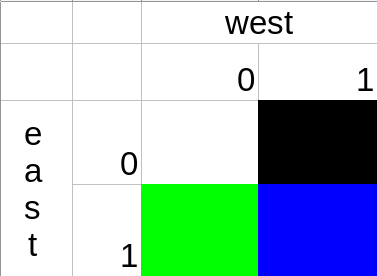
\includegraphics[width=8cm]{color_scheme}
		\label{fig:img1}
		\caption{Color scheme}
	\end{figure}
	This project uses custom LCD library written in Java. Resolution of the LCD is 17x20 and it has 4-bit color scheme. In the library implementation, memory is statically allocated so that you can feed data to one LCD and display it on another. There are 32-bit inputs on the east and west sides. Each display input only processes the upper 17 bits. To draw each row, the corresponding inputs are taken and matched against each other. If 0 is stored at the same bit position, then a white pixel is displayed. If the bit from the east input is 1 and the bit from the west input is 0 then a green pixel is drawn. If the bit from the west input is 1 and from the east input is 0, then a black pixel is drawn. If the same bit position in the east and west input is 1, then a blue pixel is displayed. Coordinates are counted from the top left.
	
\end{document}